\chapter{Validação da arquitetura} \label{cap:aplicacao_exemplo}

  Para validar a API construída, o protocolo de comunicação proposto entre a API e o módulo Matemático
  e a arquitetura proposta em geral, foram criados a aplicação cliente do Pentano e um módulo matemático
  que implementa o algoritmo k-Means para a clusterização.
  
  \begin{figure}[h!]
    \centering
    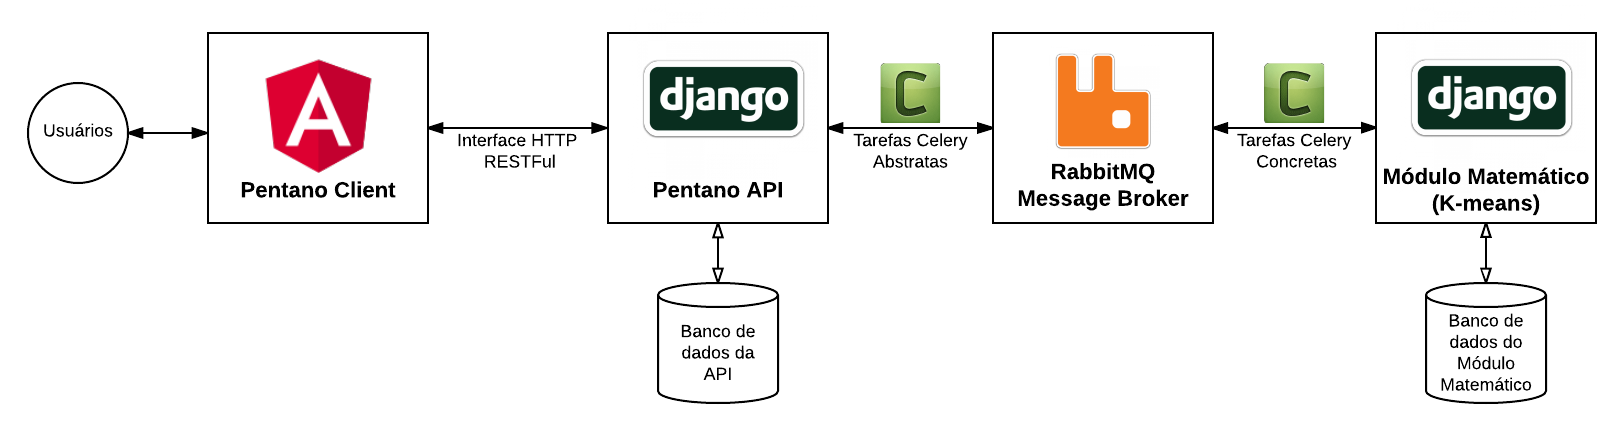
\includegraphics[scale=0.3]{figuras/whole_solution.png}
    \caption{Solução completa utilizando a arquitetura proposta.}
    \label{fig:whole_solution}
  \end{figure}
  
  A Figura \ref{fig:whole_solution} apresenta a solução completa implementada, que
  é composta por:
  
  \begin{enumerate}
      \item a aplicação cliente do Pentano, que é uma aplicação \textit{web} amigável ao usuário que fornece 
      fácil acesso aos serviços providos pela API;
      \item a API do Pentano, que fornece os serviços de autenticação e gerenciamento das conversas, comentários e votos; 
      \item uma instância do módulo matemático,
	  que fornece o serviço de clusterização para agrupar os usuários; e
      \item uma instância do RabbitMQ\footnotemark para
	  intermediar a comunicação entre a API e o módulo matemático, servindo como meio de transporte das
	  mensagens disparadas pelo Celery.
	  \footnotetext{https://www.rabbitmq.com/}
  \end{enumerate}

  Nas próximas seções são apresentados os detalhes de cada parte desta solução implementada
  para validar a arquitetura proposta.
  
%     Colocar links para os repos
  
  \section{Aplicação Cliente e API}
    
    A aplicação cliente serve como interface gráfica para os serviços de 
    gerenciamento de conversas, comentários e votos providos pela API e foi
    criada para consolidar as funcionalidades desenvolvidas e fornecer uma interface mais
    amigável para o sistema.
    
    Foram implementados todos os requisitos descritos na seção \ref{functional_requirements}
    em uma aplicação Angular 2\footnotemark para
    testar a integração com todos os \textit{endpoints} da API e demonstrar o comportamento da API.
    \footnotetext{https://angular.io/}
    
    Esta aplicação foi feita utilizando os recursos providos pelo próprio \textit{framework}, portanto
    possui uma arquitetura baseada em componentes, claramente apresentada na própria documentação do Angular \footnotemark.
    
    Resumidamente, a arquitetura consiste em uma hierarquia de componentes organizados
    em módulos independentes que se comunicam para compor a aplicação e realizar o objetivo desejado.
    Cada componente conta com um \textit{template} HTML e uma classe para gerenciar o comportamento do componente.
    Cada módulo pode possuir serviços, que são classes que encapsulam a lógica da aplicação.
    É a partir da camada de serviços que a integração com a API é realizada.
    \footnotetext{https://angular.io/guide/architecture}
    
    Quando um nova conversa, comentário ou voto são criados na aplicação cliente,
    a API é invocada para a criação do respectivo dado, que por sua vez
    notitifica o módulo matemático da ação recém ocorrida para que o mesmo possa reagir de acordo.
    Esta comunicação é feita através de tarefas do Celery e são transportadas como mensagens assíncronas
    através do RabbitMQ para o módulo matemático.
    
    Nesta implementação, ao serem criados conversas, comentários e votos, o módulo matemático apenas
    sincroniza seu banco de dados com os novos dados.
  
  \section{Módulo matemático}
  
%     - Falar sobre a escolha do Sklearn 
%     - Falar brevemente da arquitetura desenvolvida (pq isso era + trabalho do Tallys)
%     - Subir o apêndice
    
    Quando a aplicação cliente solicita os dados dos grupos de usuários de uma conversa,
    a API delega ao módulo matemático responder o dado solicitado. A partir daí o módulo
    matemático começa a trabalhar, realizando todo o processo de clusterização dos usuários
    a partir dos votos em comentários da respectiva conversa solicitada.
    
    O módulo matemático criado utiliza o algoritmo k-Means, apresentado no Capítulo \ref{cap:classificacao},
    para realizar a composição dos \textit{clusters} de usuários.
    Os detalhes dessa implementação são apresentados a seguir.

    No ``Empurrando Juntos'' a entrada para os \textit{clusters} é a combinação entre participante,  
    comentário e o voto. Essa combinação gera uma entrada de N dimensões para N comentários.
    Frequentemente antes de medir a similaridade entre os objetos é necessário
    reduzir a dimensionalidade, isso acontece, pois para espaços de alta dimensão as distâncias euclidianas
    tendem a inflar. Reduzir a dimensionalidade pode aliviar esse problema e diminuir o tempo de cálculo.
    Um dos métodos mais utilizados para realizar essa redução é a Análise de 
    Componentes Principais (PCA, do inglês) \cite{han2011data, sklearn}.

    \citeonline{mackiewicz1993principal} afirmam que a redução de dimensionalidade no PCA é
    obtida com a criação de uma nova combinação linear das variáveis que caracterizam os
    objetos estudados, satisfazendo condições matemáticas e estatísticas.
    \citeonline{shlens2014tutorial} afirma que o principal objetivo da técnica é identificar
    uma base para expressar um conjunto de dados que elimine os ruídos e revele 
    outros dados escondidos.

    \citeonline{han2011data} afirmam que o PCA 
    cria $k$ vetores ortogonais que possuem o mesmo significado que o conjunto
    de vetores inicial, porém trata-se de um conjunto menor. 

    A aplicação da técnica pode ser resumida nos seguintes passos listados abaixo.
    No final, os componentes principais restantes são uma boa aproximação dos 
    dados originais \cite{han2011data, mackiewicz1993principal, varella2008analise}: 

    \begin{enumerate}
      \item Criar uma matriz que represente os objetos estudados (n x p), onde as linhas representam cada objeto e as colunas representam as características;
      \item Criar uma matriz de covariância (p x p) com os dados normalizados, caso as unidades sejam diferentes,
	para que eles estejam dentro da mesma variação;
      \item Calcular os autovalores e autovetores da matriz de covariância, que 
      são os componentes principais.
    \end{enumerate}

    Além do PCA, foi aplicada uma técnica analítica para a definição do melhor valor para $k$, conhecida como Coeficiente de Silhueta \cite{sklearn}.

    Essa técnica tem por objetivo combinar a avaliação de coesão e separação dos \textit{clusters} por meio do cálculo de um coeficiente (o de silhueta) que 
    varia de -1 a 1 e é dado pela fórmula \ref{eq:coeficiente} \cite{tan2013data}.

    \begin{equation} \label{eq:coeficiente}
      s_{i} = \frac{(b_{i} - a_{i})}{max(a_{i}, b_{i})} \mbox{, onde:}
    \end{equation}

    {\addtolength{\leftskip}{8mm}
	i é o objeto do \textit{cluster} que está sendo analisado
	
	$a_{i}$ é a média da distância entre o objeto e todos os objetos do seu \textit{cluster}
	
	$b_{i}$ é o valor mínimo da distância entre o objeto e os demais \textit{clusters}. 
	
	      \footnotesize \indent \indent A distância entre o objeto e outro \textit{cluster} é média das distâncias entre o objeto \\ \indent \indent e todos os objetos do outro \textit{cluster}.
    }

    Um coeficiente negativo representa que o elemento está no \textit{cluster} errado, pois isso significa que a distância entre o objeto e outro \textit{cluster} 
    é menor que a distância entre o objeto e os objetos de seu \textit{cluster}. O valor ``zero'' representa que o elemento está próximo da ``borda'' do \textit{cluster}, ou seja,
    a distância entre o objeto e outros \textit{clusters} e entre o objeto e os objetos de seu \textit{cluster} é a mesma. E por fim, quanto mais próximo do valor 1, melhor
    está a distribuição dos \textit{clusters}, pois significa que o valor de $a_i$ é menor que o valor de $b_i$.

    Dessa forma, com a escolha de um intervalo de valores para $k$, como sugerido por \citeonline{han2011data} e \citeonline{sklearn}, é possível testar os valores 
    para o coeficiente de silhueta e escolher o melhor valor de $k$ dentro do intervalo. 

    \begin{figure}[bt!]
      \centering
      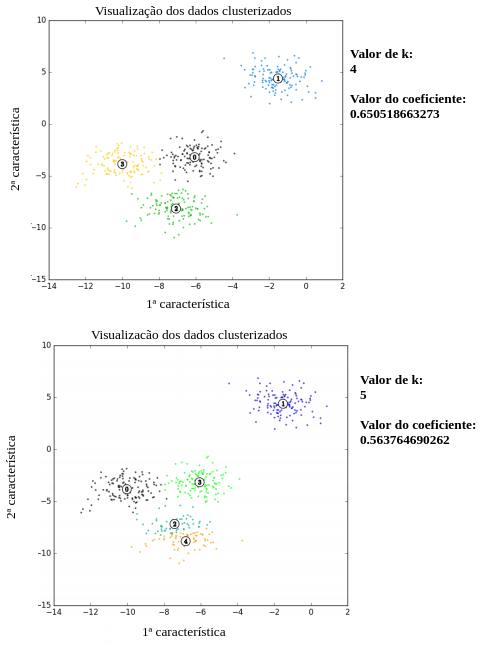
\includegraphics[scale=1]{figuras/exemplo_silhueta.png}
      \caption{Formação de \textit{clusters} utilizando K-means e seus coeficientes de silhueta. Adaptado de \citeonline{sklearn}}
      \label{fig:exemplo_silhueta}
    \end{figure}

    Na Figura \ref{fig:exemplo_silhueta} é apresentado um exemplo visual de \textit{clusters} com diferentes valores
    de $k$ e seus coeficientes de silhueta.

    Os métodos e técnicas apresentados fazem parte do algoritmo implementado no módulo de clusterização da plataforma 
    e possuem um objetivo específico.

    \begin{figure}[h!]
      \centering
      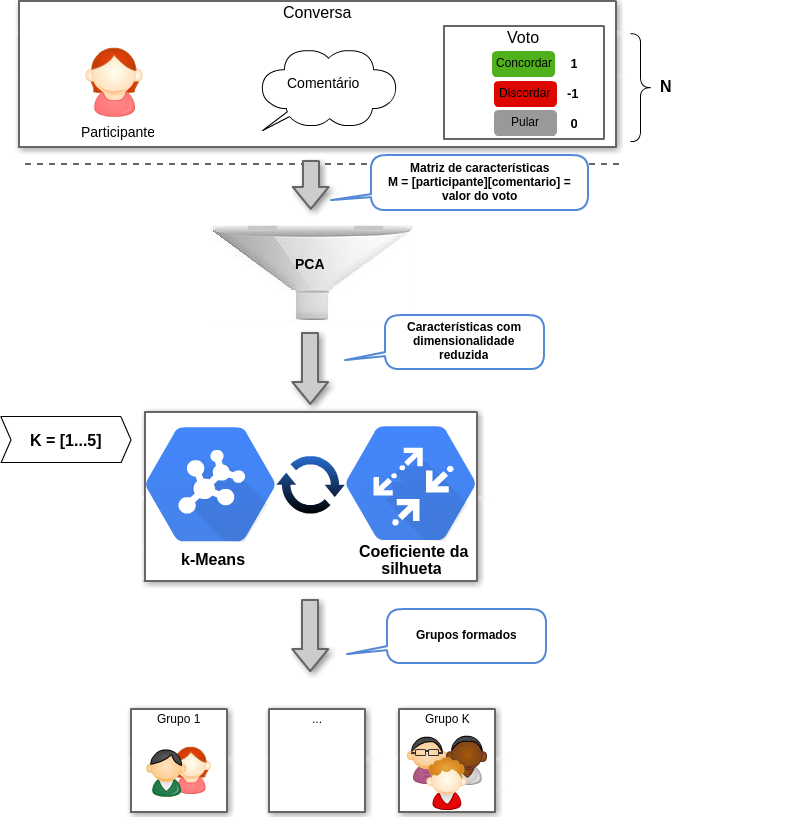
\includegraphics[scale=0.7]{figuras/resumo_clusterizao_ej.png}
      \caption{Fluxo de clusterização do ``Empurrando Juntos''}
      \label{fig:resumo_clusterizao_ej}
    \end{figure}

    Quando o usuário cria uma conversa e outros participantes realizam comentários, para cada usuário é permitido realizar votos nesse comentários.
    Atualmente, a ideia é que o voto seja concordar, discordar ou pular. 

    A cada novo voto o fluxo apresentado na Figura \ref{fig:resumo_clusterizao_ej} é
    realizado.
    Para cada conversa, os N votos realizados nos N comentários são a entrada para o módulo de clusterização, 
    gerando uma entrada de dimensão N. A partir disso, é aplicada a técnica de PCA para que
    essa dimensionalidade seja reduzida. Com os dados em duas dimensões, é aplicado o algoritmo k-Means,
    para obtenção da disposição dos grupos de pessoas. O uso da técnica é
    feito em ciclos para a descoberta do melhor valor de $k$ por meio do cálculo do coeficiente de silhueta.
    No final dos ciclos, na saída do fluxo são formados os grupos de pessoas com opiniões semelhantes, que são retornados para API.

  \section{Resultados e Discussão}
  
    - Falar do que foi possível visualizar na aplicação
    - Falar que existem outros algoritmos que o sklearn possui
    - Falar das limitações da aplicação feita
    
    Foi possível validar os serviços providos pela API implementada ao criar um cliente.